% Expanded TEC/TO package studies. This file is inserted into the ORIGINAL
% report.tex source; none of the existing sections, figures or appendices
% are deleted or replaced. All numbers use independently accepted saved states.
% No simulator or detector-transport solve is invoked by typesetting.
\clearpage
\section{Thermoelectric transport sensitivity in the current cooler}
\label{sec:current-material-sensitivity}
An operating-temperature prediction depends critically on the actual paired
P- and N-type material transport functions. The present synthetic cooler uses
the full source-leg count, ceramic spatial fields, and metal heat paths, but
its research-specimen \(S(T)\), \(\rho(T)\), and \(k(T)\) curves are not a
measured or manufacturer-qualified TEC material pair. It would therefore be
premature to quote a narrow error bar on the absolute cold-stage temperature.

To quantify the leverage of these properties, a controlled source-geometry
study changed one common P/N property factor at a time, with the original
geometry, stage count, foil connections, mounting, gas, and electrical drive
held fixed. Each point is a full 88-leg, four-ceramic nonlinear solution,
\emph{not} a scaled temperature inferred from an isolated thermocouple.
The study applied \(I_{\rm TEC}=0.400\) A, a 300 K external reservoir, 100 Pa
krypton, and a conditional auxiliary detector load obtained from
\(0.866025^2/R_{\rm die}(T)\) plus 0.500 mW absorbed heat. The illustrative
\(R_{\rm die}(T)\) law in this study is \emph{not} used to infer actual detector
performance; the gas study later in this assessment retains a strictly fixed
2.000 mW imposed heat load. Consequently the two experiment families
must not be interpreted as identical detector-loading conditions.

\begin{center}\small
\begin{tabular}{lrrr}\toprule
P/N property hypothesis & Device mount (K) & Top ceramic (K) & TEC input (W)\\\midrule
All source factors 1.00 & 218.900 & 218.807 & 0.595668\\
Thermal conductivity \(\times0.80\) & 207.812 & 207.716 & 0.616656\\
Thermal conductivity \(\times1.20\) & 227.627 & 227.536 & 0.579393\\
Seebeck coefficient \(\times0.90\) & 225.833 & 225.741 & 0.562663\\
Seebeck coefficient \(\times1.10\) & 212.515 & 212.420 & 0.631764\\
Electrical resistivity \(\times0.80\) & 216.563 & 216.470 & 0.523689\\
Electrical resistivity \(\times1.20\) & 221.313 & 221.221 & 0.668943\\\bottomrule
\end{tabular}
\end{center}

Under the \emph{selected, unequal} factor intervals, the total device-mount
temperature endpoint spans are \(19.815\) K for \(k\), \(13.318\) K for
\(S\), and \(4.750\) K for \(\rho\), respectively. The ranking is an
engineering screening result, \textbf{not} a statistical sensitivity ranking:
the factor ranges are deliberately different, and independently modifying
only one material property can be physically incompatible with a real
thermoelectric grade.
\begin{center}
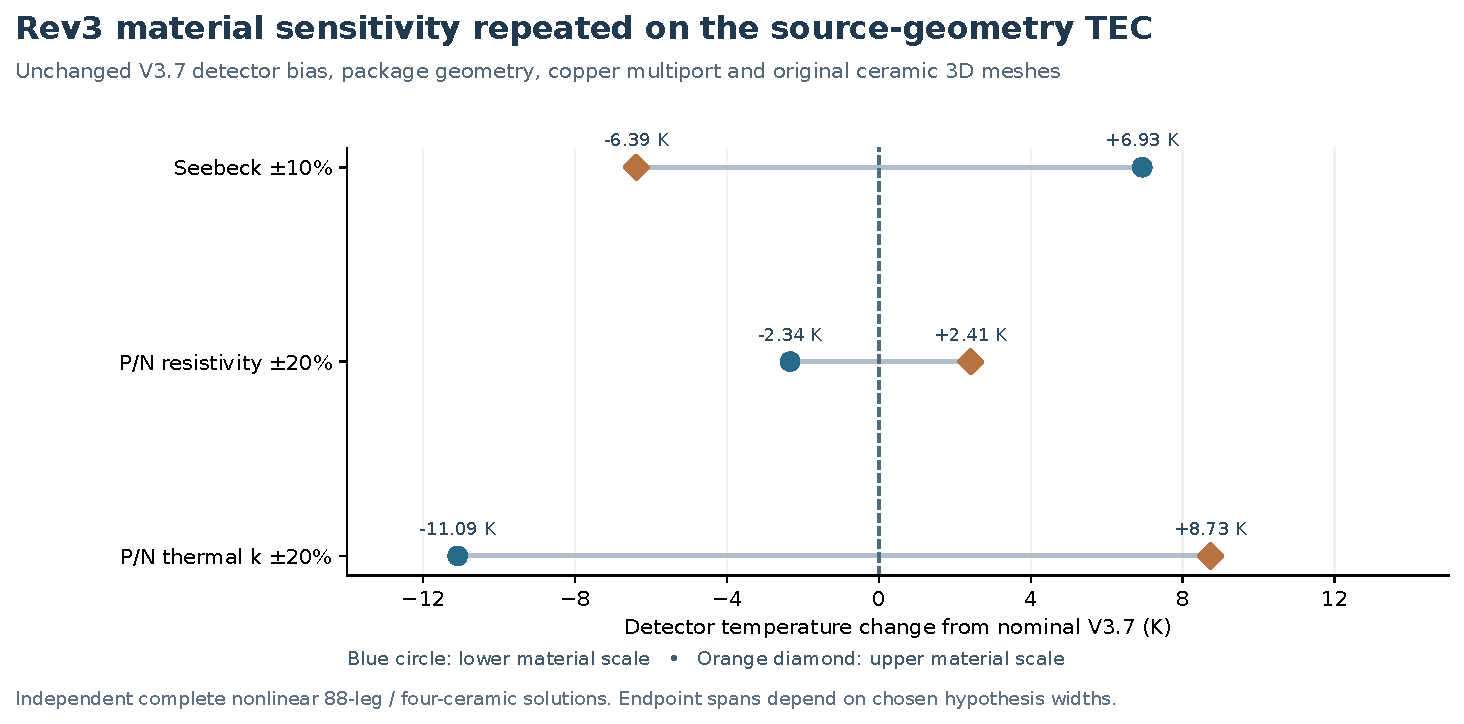
\includegraphics[width=.95\linewidth,height=.38\textheight,keepaspectratio]{figures/v38_source_material_response.pdf}
\par\vspace{1mm}{\small\textit{Figure \the\numexpr\value{figure}+1\relax.} Independently solved P/N
transport variations on the current full TEC/TO thermal architecture.
Source-property factor ranges are hypotheses, not production tolerances.}
\end{center}\stepcounter{figure}

\clearpage
\section{Package mounting and power required to hold a cold temperature}
\label{sec:mounting-and-matched-power}
Even with a fixed 300 K external reservoir, the hot ceramic is not
constrained to 300 K. Heat is rejected through an assumed finite package
mounting resistance. The nominal current reference uses
\(R_{\rm external}=4.833387\ {\rm K/W}\); the two controlled hypotheses add
5 or 10 K/W \emph{on top of} that reference. The combined
source-ceramic and 88-leg transport state was re-solved for each case, with
the same stated reference detector thermal-input law and TEC current.

\begin{center}\small
\begin{tabular}{rrrr}\toprule
Additional \(R_{\rm mount}\) & Total \(R_{\rm external}\) & Device mount \(T\) & TEC input\\
(K/W) & (K/W) & (K) & (W)\\\midrule
0 & 4.833387 & 218.900 & 0.595668\\
5 & 9.833387 & 220.393 & 0.604935\\
10 & 14.833387 & 221.856 & 0.613656\\\bottomrule
\end{tabular}
\end{center}
The fixed-current temperature penalties are \(+1.493\) K and
\(+2.956\) K for the added 5 and 10 K/W, respectively. Mounting resistance
is a package design variable and should not be confused with the cooler's
intrinsic material heat lift.

\begin{center}
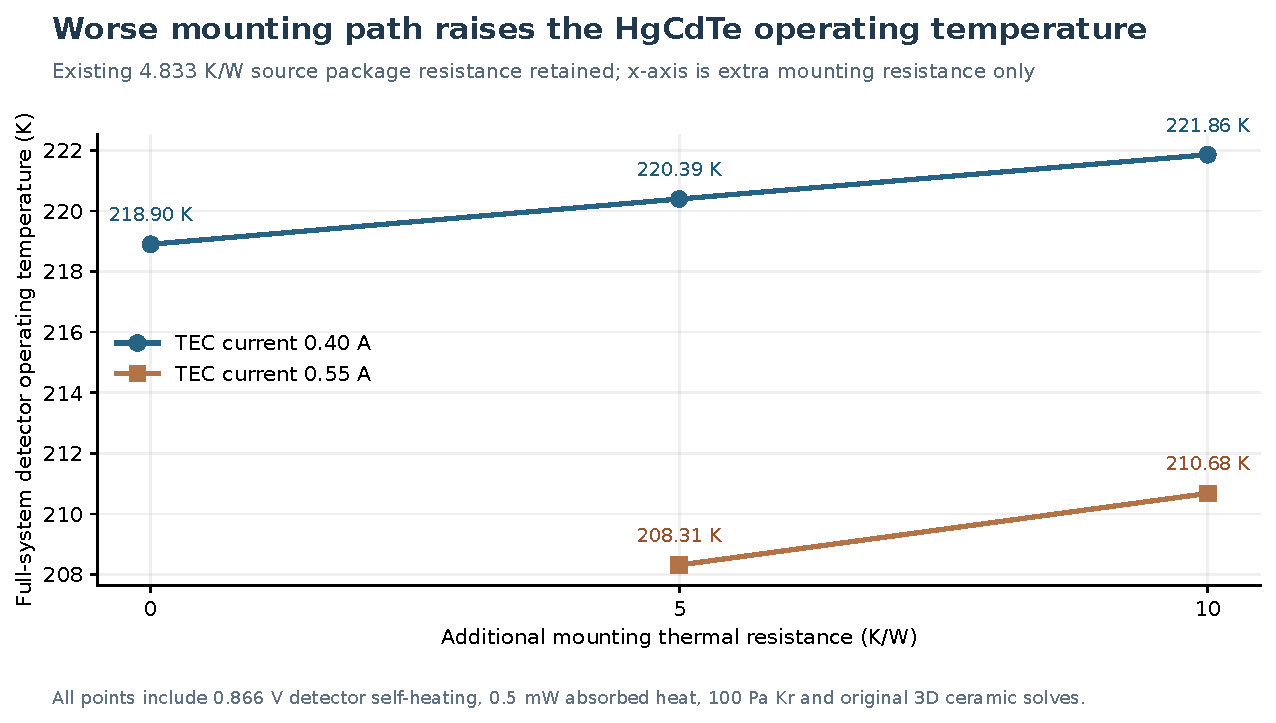
\includegraphics[width=.92\linewidth,height=.40\textheight,keepaspectratio]{figures/v38_package_sink_temperature.pdf}
\par\vspace{1mm}{\small\textit{Figure \the\numexpr\value{figure}+1\relax.}
The finite external mounting path changes the nonlinear whole-device
temperature distribution; the detector is not assigned a temperature rise
algebraically.}
\end{center}\stepcounter{figure}

A more practical procurement and instrument-design question is how
much additional electrical power is required to \emph{recover the same}
operating temperature when mounting quality deteriorates. Two new
registered, independently audited source solutions were obtained
after a bounded current bracket and one numerical correction.
These are \emph{actual} full-system solutions, not interpolated electric
power values.
\begin{center}\small
\begin{tabular}{rrrrr}\toprule
Extra \(R\) (K/W) & TEC \(I\) (A) & Device mount (K) & Input (W) & Power penalty\\\midrule
0 & 0.400000 & 218.900024 & 0.595668 & Reference\\
5 & 0.415286 & 218.892717 & 0.648375 & +8.85\%\\
10 & 0.433174 & 218.868845 & 0.712481 & +19.61\%\\\bottomrule
\end{tabular}
\end{center}
The maximum matched-temperature departure is just \(0.0312\) K.
The \(+10\) K/W mounting case demands approximately
\(116.8\) mW more \emph{TEC terminal power} to deliver essentially
the same device-platform temperature, under the chosen boundary
and material assumptions.

\clearpage
\begin{center}
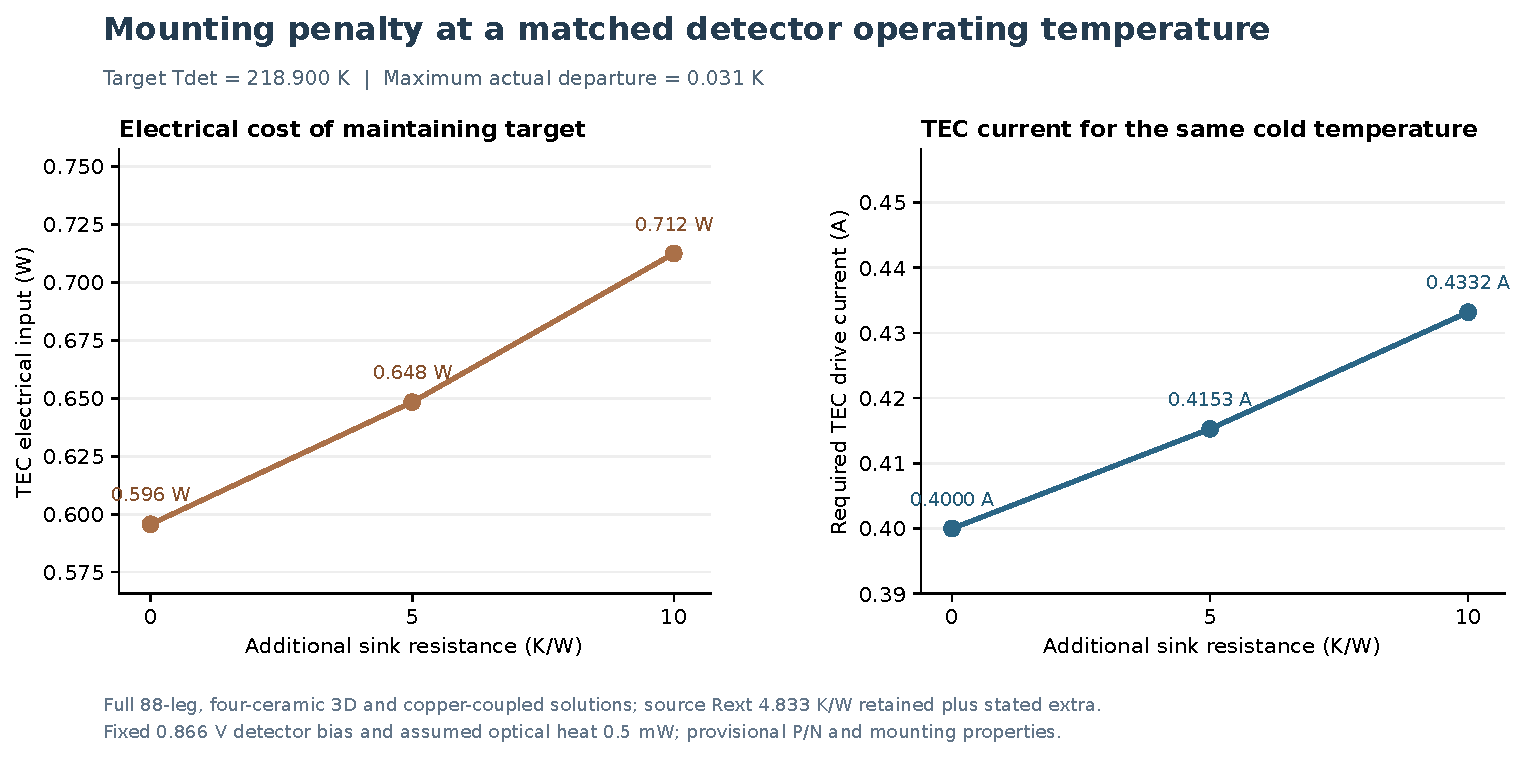
\includegraphics[width=.97\linewidth,height=.59\textheight,keepaspectratio]{figures/v38_matched_detector_temperature_power.pdf}
\par\vspace{2mm}{\small\textit{Figure \the\numexpr\value{figure}+1\relax.}
Calculated TEC current and terminal input required to maintain
near-equal mounting temperature as external resistance increases.
The comparison is not a measured OEM power rating or a global optimum.}
\end{center}\stepcounter{figure}

\subsection{Source-property validity above 300 K}
At the reference mounting condition the hot ceramic reaches about
303.8 K; with an additional 10 K/W it reaches about 309.5 K. The P/N
research curves have published markers through 300 K only. A separate
six-run continuation check held the original 40--300 K curves exactly fixed,
while assigning \(0\), \(25\), or \(100\%\) of the final source-curve
tangent beyond 300 K. Across those hypotheses the device temperature
spanned only \(0.0170\) K at nominal mounting and \(0.0782\) K under
the worsened mounting condition. The corresponding total TEC input-power
spans were \(0.545\) and \(3.115\) mW.

This result helps distinguish a \emph{particular extrapolation parameter}
from the much larger unqualified \emph{bulk P/N material grade} question.
It does not demonstrate that any of the three continuations is physically
correct, nor does it provide a statistical uncertainty interval.

\textbf{Engineering interpretation.}
Improving material-grade evidence and the mechanical/thermal TO mounting
interface should precede an expensive broad numerical sweep of speculative
high-temperature extrapolation functions. For any colder operating point,
state current, terminal voltage, heat load, source-temperature coverage,
mounting resistance, and the relevant electrical-power budget.

\clearpage
\section{Effect of cavity backfill on the TEC top stage}
\label{sec:package-backfill-current}
The packaged cooler is also subjected to a potentially substantial heat
leak from warm internal surfaces. A controlled eight-case study has now
re-solved the \emph{same} source-based TEC with rarefied-to-continuum
Kr, Ar and N$_2$ backfill conditions. To separate cavity transport from
detector-specific electronics, these simulations use a fixed
\(\boxed{Q_{\rm die}=2.000\ {\rm mW}}\) rather than an
electrical-resistance or optical absorption calculation.
The principal comparison holds
\(I_{\rm TEC}=0.400\ {\rm A}\) and external temperature 300 K.

\begin{center}\small
\begin{tabular}{lrrrr}\toprule
Backfill & Top ceramic & Device mount & Gas heat & TEC power\\
 & (K) & (K) & (mW) & (W)\\\midrule
Vacuum, gas off & 218.353 & 218.437 & 0.000 & 0.596111\\
Kr, 100 Pa & 218.807 & 218.900 & 3.420 & 0.595668\\
Kr, 30 kPa & 218.845 & 218.939 & 3.724 & 0.595630\\
Kr, 101.325 kPa & 218.845 & 218.939 & 3.725 & 0.595630\\
Ar, 30 kPa & 219.277 & 219.380 & 6.966 & 0.595209\\
N$_2$, 30 kPa & 219.703 & 219.815 & 10.170 & 0.594792\\
N$_2$, 101.325 kPa & 219.703 & 219.815 & 10.172 & 0.594792\\\bottomrule
\end{tabular}
\end{center}

At the same 30 kPa nominal pressure, nitrogen is \(0.8753\) K
warmer than krypton at the device mounting node and imports an
additional \(6.446\) mW of gas heat. Argon lies between the two.
Disabling gas conduction entirely gives a \(0.4634\) K cooler
mounting condition than 100 Pa Kr, while leaving solid and radiative
conduction active. No numerical result is assigned to a manufacturer
or a known production-gas recipe.

\begin{center}
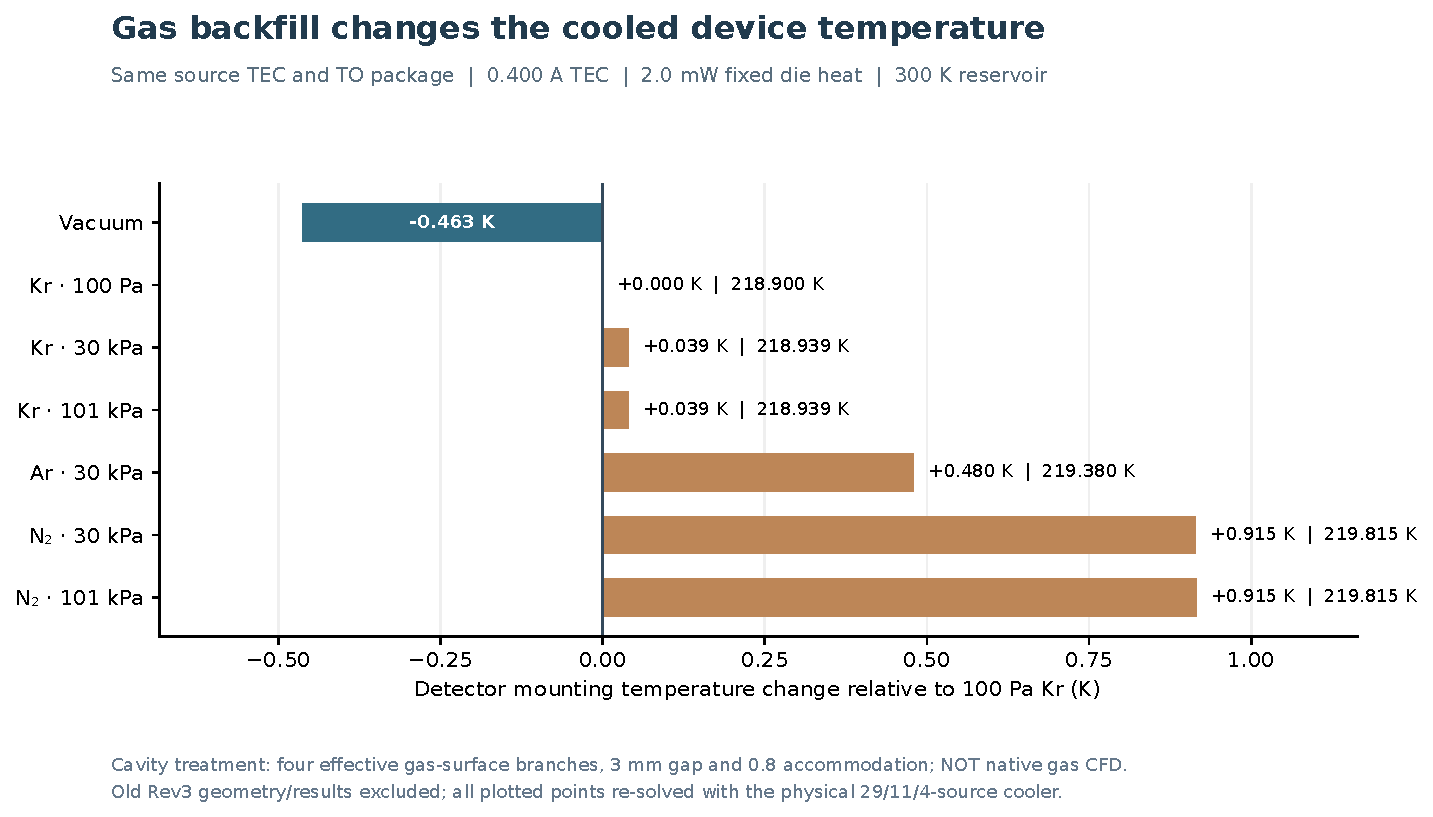
\includegraphics[width=.95\linewidth,height=.42\textheight,keepaspectratio]{figures/v311_backfill_species_pressure_cold_temperature.pdf}
\par\vspace{1mm}{\small\textit{Figure \the\numexpr\value{figure}+1\relax.}
Backfill gas and pressure sensitivity of the
device-side mounting temperature. The top TEC ceramic is a distinct
lower-temperature node; both are listed in the accompanying table.}
\end{center}\stepcounter{figure}

\clearpage
\section{Gas heat-transfer mechanism and its uncertainty}
\label{sec:gas-model-fidelity}
The current cavity calculation is a \emph{reduced effective-gap}
conduction model, not a finite-volume or finite-element solution of
gas transport around all 88 exposed thermoelectric legs. For
a warm enclosure surface and cold branch \(i\),
\[
Q_{{\rm gas},i}=G_{{\rm gas},i}(T_{\rm env}-T_i), \qquad
G_{{\rm gas},i}=
\frac{k_{\rm gas}(\overline{T})A_i}{
g+2\ell_{\rm jump}(p,\overline{T},\alpha)}.
\]
Here \(g=3\) mm is an \emph{assumed} effective gap, the thermal
accommodation coefficient is \(\alpha=0.8\), and the four
assigned branch areas are \(12.60,\ 8.68,\ 4.76,\ 1.00\ {\rm mm^2}\).
Temperature-dependent tabulated Kr, Ar and N$_2$ conductivities,
an Eucken-based viscosity estimate, and a temperature-jump
rarefaction correction determine each conductance.

\begin{center}
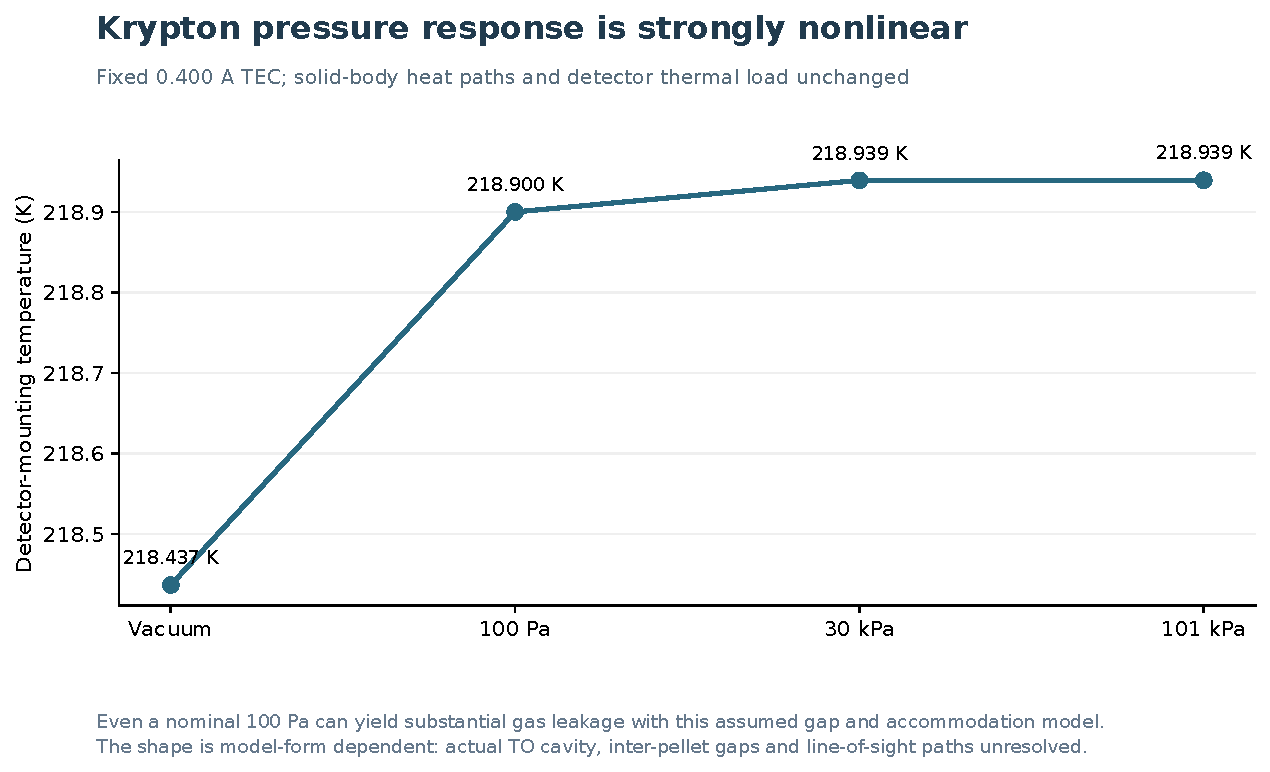
\includegraphics[width=.91\linewidth,height=.42\textheight,keepaspectratio]{figures/v311_krypton_pressure_sensitivity.pdf}
\par\vspace{1mm}{\small\textit{Figure \the\numexpr\value{figure}+1\relax.}
Discrete rarefied-gas/pressure scenarios for Kr in the
declared effective-gap model. Connecting lines are guides only,
not a measured or independently verified continuum response curve.}
\end{center}\stepcounter{figure}

Under this particular model, raising Kr pressure
from 100 Pa to 30 kPa adds just \(0.03930\) K to the device temperature;
raising it from 30 kPa to 101.325 kPa adds only \(0.00010\) K.
This apparent saturation is largely a consequence of the chosen
effective gap, warm-area mapping, and accommodation law.
The physically available narrow gaps between
\(0.40\)-mm-wide pellets spaced on a \(0.58\)-mm pitch
are not represented as independently exposed gas channels.
A more faithful cavity model could change both the pressure
transition and the gas species ranking. The present data
\textbf{must not} be used to claim pressure is unimportant
in an actual TO package at 100 Pa.

\clearpage
\section{Thermal loading, electrical demand, and engineering optimization}
\label{sec:current-design-optimization}
Changing TEC drive current is not a gas effect, but it sets the
trade-off between cold temperature and electrical power.
A separately solved case at \(I_{\rm TEC}=0.550\) A and
30 kPa Kr, with the same 2 mW die heat and 300 K reservoir, gives
\[
T_{\rm top\ ceramic}=205.931\ {\rm K},\quad
T_{\rm die}=206.032\ {\rm K},\quad
P_{\rm TEC}=1.06462\ {\rm W}.
\]
Relative to 0.400 A at 30 kPa Kr this lowers device
temperature by \(12.908\) K while raising terminal input by
\(0.469\) W. Such a trade-off is useful only when a
real operating envelope and safe current/voltage limits
are independently established.

\subsection{Prioritize physical knobs before creating a broad optimization surface}
The existing new-architecture studies support the following
\emph{engineering experiments}, with their distinction between
real geometric variables and screening assumptions preserved.

\begin{center}\small
\begin{tabularx}{\linewidth}{p{42mm}p{33mm}X}\toprule
Construction or operating knob & Existing conditional effect & Next physical qualification\\\midrule
P/N material transport \(k,S,\rho\) &
\(19.8,\ 13.3,\ 4.75\) K source-factor spans &
Real matched P/N grade and correlated properties\\
External mounting resistance &
+2.96 K at +10 K/W, fixed 0.4 A &
TO contact patch, heat spreader and interface pressure\\
Formed-Cu foil/joint thermal path &
6.276 K for an \emph{extreme} contact hypothesis &
Solder/plating area, Cu bending, electrical resistance and current crowding\\
Gas species, 30 kPa, Kr to N$_2$ &
+0.875 K &
Native cavity exposure and inter-pellet gap distribution\\
Detector prescribed load, 1--6 mW &
About 1.56 K span at 0.4 A &
Define die/power budget, attach and carrier conductivity\\
TEC drive current, 0.4 to 0.55 A at 30 kPa Kr &
\(-12.908\) K at \(+0.469\) W &
Rated current, lifetime and allowable package dissipation\\\bottomrule
\end{tabularx}
\end{center}

A physically credible optimization of top-stage temperature should vary
the pellet area \(A\), height \(L\), stage placement, current and
source-grounded package thermal boundaries \emph{jointly}, subject to
specified electrical and mechanical constraints:
\[
\min\,T_{\rm top}(I,A,L,Q_{\rm die},T_{\rm sink},
R_{\rm mount},p_{\rm gas},\ldots).
\]
A transport-only \(A,L\) sweep can isolate competing
\(R_{\rm leg}\sim \rho L/A\) and \(K_{\rm leg}\sim kA/L\)
effects. It cannot by itself be called a fabricated
pellet-geometry variant: changing width or height also changes
solder pad area, foil contact location, ceramic spacing,
interleg gas gaps and insulation clearance.

\subsection{Evidence quality and outstanding physical work}
All eight gas cases and the material/mounting studies archive
original 88-leg nonlinear states, source native four-ceramic
3D nodal fields, input registrations and independent audits.
The eight gas cases all pass direct independently
reconstructed gas conductance, source Cu/lead Joule,
three-stage and global heat balances; their maximum
global energy residual is below \(2\times10^{-9}\) W.
This demonstrates conservation \emph{of the declared model}.
It does not identify actual P/N pellet batches,
solder thermal impedances, or exposed package gas
paths, nor does it establish a full multi-material
430-domain current and thermal PDE.

The next high-value releases should therefore be:
a source-grounded pellet width/height feasibility screen,
a native exposed-surface cavity network,
and a quantified TO mounting/contact construction
study. For each, report \emph{top ceramic temperature},
die mounting temperature, thermoelectric input,
package rejected heat, and individual component
heat-flow budgets. Semiconductor signal/noise and
photodetection belong to the separate specialist model;
they are not necessary to answer these package
thermal-design questions.
\clearpage
